\documentclass{article} % For LaTeX2e
\usepackage{iclr2022_conference,times}
\usepackage{graphicx}
% Optional math commands from https://github.com/goodfeli/dlbook_notation.
%%%%% NEW MATH DEFINITIONS %%%%%

\usepackage{amsmath,amsfonts,bm}

% Mark sections of captions for referring to divisions of figures
\newcommand{\figleft}{{\em (Left)}}
\newcommand{\figcenter}{{\em (Center)}}
\newcommand{\figright}{{\em (Right)}}
\newcommand{\figtop}{{\em (Top)}}
\newcommand{\figbottom}{{\em (Bottom)}}
\newcommand{\captiona}{{\em (a)}}
\newcommand{\captionb}{{\em (b)}}
\newcommand{\captionc}{{\em (c)}}
\newcommand{\captiond}{{\em (d)}}

% Highlight a newly defined term
\newcommand{\newterm}[1]{{\bf #1}}


% Figure reference, lower-case.
\def\figref#1{figure~\ref{#1}}
% Figure reference, capital. For start of sentence
\def\Figref#1{Figure~\ref{#1}}
\def\twofigref#1#2{figures \ref{#1} and \ref{#2}}
\def\quadfigref#1#2#3#4{figures \ref{#1}, \ref{#2}, \ref{#3} and \ref{#4}}
% Section reference, lower-case.
\def\secref#1{section~\ref{#1}}
% Section reference, capital.
\def\Secref#1{Section~\ref{#1}}
% Reference to two sections.
\def\twosecrefs#1#2{sections \ref{#1} and \ref{#2}}
% Reference to three sections.
\def\secrefs#1#2#3{sections \ref{#1}, \ref{#2} and \ref{#3}}
% Reference to an equation, lower-case.
\def\eqref#1{equation~\ref{#1}}
% Reference to an equation, upper case
\def\Eqref#1{Equation~\ref{#1}}
% A raw reference to an equation---avoid using if possible
\def\plaineqref#1{\ref{#1}}
% Reference to a chapter, lower-case.
\def\chapref#1{chapter~\ref{#1}}
% Reference to an equation, upper case.
\def\Chapref#1{Chapter~\ref{#1}}
% Reference to a range of chapters
\def\rangechapref#1#2{chapters\ref{#1}--\ref{#2}}
% Reference to an algorithm, lower-case.
\def\algref#1{algorithm~\ref{#1}}
% Reference to an algorithm, upper case.
\def\Algref#1{Algorithm~\ref{#1}}
\def\twoalgref#1#2{algorithms \ref{#1} and \ref{#2}}
\def\Twoalgref#1#2{Algorithms \ref{#1} and \ref{#2}}
% Reference to a part, lower case
\def\partref#1{part~\ref{#1}}
% Reference to a part, upper case
\def\Partref#1{Part~\ref{#1}}
\def\twopartref#1#2{parts \ref{#1} and \ref{#2}}

\def\ceil#1{\lceil #1 \rceil}
\def\floor#1{\lfloor #1 \rfloor}
\def\1{\bm{1}}
\newcommand{\train}{\mathcal{D}}
\newcommand{\valid}{\mathcal{D_{\mathrm{valid}}}}
\newcommand{\test}{\mathcal{D_{\mathrm{test}}}}

\def\eps{{\epsilon}}


% Random variables
\def\reta{{\textnormal{$\eta$}}}
\def\ra{{\textnormal{a}}}
\def\rb{{\textnormal{b}}}
\def\rc{{\textnormal{c}}}
\def\rd{{\textnormal{d}}}
\def\re{{\textnormal{e}}}
\def\rf{{\textnormal{f}}}
\def\rg{{\textnormal{g}}}
\def\rh{{\textnormal{h}}}
\def\ri{{\textnormal{i}}}
\def\rj{{\textnormal{j}}}
\def\rk{{\textnormal{k}}}
\def\rl{{\textnormal{l}}}
% rm is already a command, just don't name any random variables m
\def\rn{{\textnormal{n}}}
\def\ro{{\textnormal{o}}}
\def\rp{{\textnormal{p}}}
\def\rq{{\textnormal{q}}}
\def\rr{{\textnormal{r}}}
\def\rs{{\textnormal{s}}}
\def\rt{{\textnormal{t}}}
\def\ru{{\textnormal{u}}}
\def\rv{{\textnormal{v}}}
\def\rw{{\textnormal{w}}}
\def\rx{{\textnormal{x}}}
\def\ry{{\textnormal{y}}}
\def\rz{{\textnormal{z}}}

% Random vectors
\def\rvepsilon{{\mathbf{\epsilon}}}
\def\rvtheta{{\mathbf{\theta}}}
\def\rva{{\mathbf{a}}}
\def\rvb{{\mathbf{b}}}
\def\rvc{{\mathbf{c}}}
\def\rvd{{\mathbf{d}}}
\def\rve{{\mathbf{e}}}
\def\rvf{{\mathbf{f}}}
\def\rvg{{\mathbf{g}}}
\def\rvh{{\mathbf{h}}}
\def\rvu{{\mathbf{i}}}
\def\rvj{{\mathbf{j}}}
\def\rvk{{\mathbf{k}}}
\def\rvl{{\mathbf{l}}}
\def\rvm{{\mathbf{m}}}
\def\rvn{{\mathbf{n}}}
\def\rvo{{\mathbf{o}}}
\def\rvp{{\mathbf{p}}}
\def\rvq{{\mathbf{q}}}
\def\rvr{{\mathbf{r}}}
\def\rvs{{\mathbf{s}}}
\def\rvt{{\mathbf{t}}}
\def\rvu{{\mathbf{u}}}
\def\rvv{{\mathbf{v}}}
\def\rvw{{\mathbf{w}}}
\def\rvx{{\mathbf{x}}}
\def\rvy{{\mathbf{y}}}
\def\rvz{{\mathbf{z}}}

% Elements of random vectors
\def\erva{{\textnormal{a}}}
\def\ervb{{\textnormal{b}}}
\def\ervc{{\textnormal{c}}}
\def\ervd{{\textnormal{d}}}
\def\erve{{\textnormal{e}}}
\def\ervf{{\textnormal{f}}}
\def\ervg{{\textnormal{g}}}
\def\ervh{{\textnormal{h}}}
\def\ervi{{\textnormal{i}}}
\def\ervj{{\textnormal{j}}}
\def\ervk{{\textnormal{k}}}
\def\ervl{{\textnormal{l}}}
\def\ervm{{\textnormal{m}}}
\def\ervn{{\textnormal{n}}}
\def\ervo{{\textnormal{o}}}
\def\ervp{{\textnormal{p}}}
\def\ervq{{\textnormal{q}}}
\def\ervr{{\textnormal{r}}}
\def\ervs{{\textnormal{s}}}
\def\ervt{{\textnormal{t}}}
\def\ervu{{\textnormal{u}}}
\def\ervv{{\textnormal{v}}}
\def\ervw{{\textnormal{w}}}
\def\ervx{{\textnormal{x}}}
\def\ervy{{\textnormal{y}}}
\def\ervz{{\textnormal{z}}}

% Random matrices
\def\rmA{{\mathbf{A}}}
\def\rmB{{\mathbf{B}}}
\def\rmC{{\mathbf{C}}}
\def\rmD{{\mathbf{D}}}
\def\rmE{{\mathbf{E}}}
\def\rmF{{\mathbf{F}}}
\def\rmG{{\mathbf{G}}}
\def\rmH{{\mathbf{H}}}
\def\rmI{{\mathbf{I}}}
\def\rmJ{{\mathbf{J}}}
\def\rmK{{\mathbf{K}}}
\def\rmL{{\mathbf{L}}}
\def\rmM{{\mathbf{M}}}
\def\rmN{{\mathbf{N}}}
\def\rmO{{\mathbf{O}}}
\def\rmP{{\mathbf{P}}}
\def\rmQ{{\mathbf{Q}}}
\def\rmR{{\mathbf{R}}}
\def\rmS{{\mathbf{S}}}
\def\rmT{{\mathbf{T}}}
\def\rmU{{\mathbf{U}}}
\def\rmV{{\mathbf{V}}}
\def\rmW{{\mathbf{W}}}
\def\rmX{{\mathbf{X}}}
\def\rmY{{\mathbf{Y}}}
\def\rmZ{{\mathbf{Z}}}

% Elements of random matrices
\def\ermA{{\textnormal{A}}}
\def\ermB{{\textnormal{B}}}
\def\ermC{{\textnormal{C}}}
\def\ermD{{\textnormal{D}}}
\def\ermE{{\textnormal{E}}}
\def\ermF{{\textnormal{F}}}
\def\ermG{{\textnormal{G}}}
\def\ermH{{\textnormal{H}}}
\def\ermI{{\textnormal{I}}}
\def\ermJ{{\textnormal{J}}}
\def\ermK{{\textnormal{K}}}
\def\ermL{{\textnormal{L}}}
\def\ermM{{\textnormal{M}}}
\def\ermN{{\textnormal{N}}}
\def\ermO{{\textnormal{O}}}
\def\ermP{{\textnormal{P}}}
\def\ermQ{{\textnormal{Q}}}
\def\ermR{{\textnormal{R}}}
\def\ermS{{\textnormal{S}}}
\def\ermT{{\textnormal{T}}}
\def\ermU{{\textnormal{U}}}
\def\ermV{{\textnormal{V}}}
\def\ermW{{\textnormal{W}}}
\def\ermX{{\textnormal{X}}}
\def\ermY{{\textnormal{Y}}}
\def\ermZ{{\textnormal{Z}}}

% Vectors
\def\vzero{{\bm{0}}}
\def\vone{{\bm{1}}}
\def\vmu{{\bm{\mu}}}
\def\vtheta{{\bm{\theta}}}
\def\va{{\bm{a}}}
\def\vb{{\bm{b}}}
\def\vc{{\bm{c}}}
\def\vd{{\bm{d}}}
\def\ve{{\bm{e}}}
\def\vf{{\bm{f}}}
\def\vg{{\bm{g}}}
\def\vh{{\bm{h}}}
\def\vi{{\bm{i}}}
\def\vj{{\bm{j}}}
\def\vk{{\bm{k}}}
\def\vl{{\bm{l}}}
\def\vm{{\bm{m}}}
\def\vn{{\bm{n}}}
\def\vo{{\bm{o}}}
\def\vp{{\bm{p}}}
\def\vq{{\bm{q}}}
\def\vr{{\bm{r}}}
\def\vs{{\bm{s}}}
\def\vt{{\bm{t}}}
\def\vu{{\bm{u}}}
\def\vv{{\bm{v}}}
\def\vw{{\bm{w}}}
\def\vx{{\bm{x}}}
\def\vy{{\bm{y}}}
\def\vz{{\bm{z}}}

% Elements of vectors
\def\evalpha{{\alpha}}
\def\evbeta{{\beta}}
\def\evepsilon{{\epsilon}}
\def\evlambda{{\lambda}}
\def\evomega{{\omega}}
\def\evmu{{\mu}}
\def\evpsi{{\psi}}
\def\evsigma{{\sigma}}
\def\evtheta{{\theta}}
\def\eva{{a}}
\def\evb{{b}}
\def\evc{{c}}
\def\evd{{d}}
\def\eve{{e}}
\def\evf{{f}}
\def\evg{{g}}
\def\evh{{h}}
\def\evi{{i}}
\def\evj{{j}}
\def\evk{{k}}
\def\evl{{l}}
\def\evm{{m}}
\def\evn{{n}}
\def\evo{{o}}
\def\evp{{p}}
\def\evq{{q}}
\def\evr{{r}}
\def\evs{{s}}
\def\evt{{t}}
\def\evu{{u}}
\def\evv{{v}}
\def\evw{{w}}
\def\evx{{x}}
\def\evy{{y}}
\def\evz{{z}}

% Matrix
\def\mA{{\bm{A}}}
\def\mB{{\bm{B}}}
\def\mC{{\bm{C}}}
\def\mD{{\bm{D}}}
\def\mE{{\bm{E}}}
\def\mF{{\bm{F}}}
\def\mG{{\bm{G}}}
\def\mH{{\bm{H}}}
\def\mI{{\bm{I}}}
\def\mJ{{\bm{J}}}
\def\mK{{\bm{K}}}
\def\mL{{\bm{L}}}
\def\mM{{\bm{M}}}
\def\mN{{\bm{N}}}
\def\mO{{\bm{O}}}
\def\mP{{\bm{P}}}
\def\mQ{{\bm{Q}}}
\def\mR{{\bm{R}}}
\def\mS{{\bm{S}}}
\def\mT{{\bm{T}}}
\def\mU{{\bm{U}}}
\def\mV{{\bm{V}}}
\def\mW{{\bm{W}}}
\def\mX{{\bm{X}}}
\def\mY{{\bm{Y}}}
\def\mZ{{\bm{Z}}}
\def\mBeta{{\bm{\beta}}}
\def\mPhi{{\bm{\Phi}}}
\def\mLambda{{\bm{\Lambda}}}
\def\mSigma{{\bm{\Sigma}}}

% Tensor
\DeclareMathAlphabet{\mathsfit}{\encodingdefault}{\sfdefault}{m}{sl}
\SetMathAlphabet{\mathsfit}{bold}{\encodingdefault}{\sfdefault}{bx}{n}
\newcommand{\tens}[1]{\bm{\mathsfit{#1}}}
\def\tA{{\tens{A}}}
\def\tB{{\tens{B}}}
\def\tC{{\tens{C}}}
\def\tD{{\tens{D}}}
\def\tE{{\tens{E}}}
\def\tF{{\tens{F}}}
\def\tG{{\tens{G}}}
\def\tH{{\tens{H}}}
\def\tI{{\tens{I}}}
\def\tJ{{\tens{J}}}
\def\tK{{\tens{K}}}
\def\tL{{\tens{L}}}
\def\tM{{\tens{M}}}
\def\tN{{\tens{N}}}
\def\tO{{\tens{O}}}
\def\tP{{\tens{P}}}
\def\tQ{{\tens{Q}}}
\def\tR{{\tens{R}}}
\def\tS{{\tens{S}}}
\def\tT{{\tens{T}}}
\def\tU{{\tens{U}}}
\def\tV{{\tens{V}}}
\def\tW{{\tens{W}}}
\def\tX{{\tens{X}}}
\def\tY{{\tens{Y}}}
\def\tZ{{\tens{Z}}}


% Graph
\def\gA{{\mathcal{A}}}
\def\gB{{\mathcal{B}}}
\def\gC{{\mathcal{C}}}
\def\gD{{\mathcal{D}}}
\def\gE{{\mathcal{E}}}
\def\gF{{\mathcal{F}}}
\def\gG{{\mathcal{G}}}
\def\gH{{\mathcal{H}}}
\def\gI{{\mathcal{I}}}
\def\gJ{{\mathcal{J}}}
\def\gK{{\mathcal{K}}}
\def\gL{{\mathcal{L}}}
\def\gM{{\mathcal{M}}}
\def\gN{{\mathcal{N}}}
\def\gO{{\mathcal{O}}}
\def\gP{{\mathcal{P}}}
\def\gQ{{\mathcal{Q}}}
\def\gR{{\mathcal{R}}}
\def\gS{{\mathcal{S}}}
\def\gT{{\mathcal{T}}}
\def\gU{{\mathcal{U}}}
\def\gV{{\mathcal{V}}}
\def\gW{{\mathcal{W}}}
\def\gX{{\mathcal{X}}}
\def\gY{{\mathcal{Y}}}
\def\gZ{{\mathcal{Z}}}

% Sets
\def\sA{{\mathbb{A}}}
\def\sB{{\mathbb{B}}}
\def\sC{{\mathbb{C}}}
\def\sD{{\mathbb{D}}}
% Don't use a set called E, because this would be the same as our symbol
% for expectation.
\def\sF{{\mathbb{F}}}
\def\sG{{\mathbb{G}}}
\def\sH{{\mathbb{H}}}
\def\sI{{\mathbb{I}}}
\def\sJ{{\mathbb{J}}}
\def\sK{{\mathbb{K}}}
\def\sL{{\mathbb{L}}}
\def\sM{{\mathbb{M}}}
\def\sN{{\mathbb{N}}}
\def\sO{{\mathbb{O}}}
\def\sP{{\mathbb{P}}}
\def\sQ{{\mathbb{Q}}}
\def\sR{{\mathbb{R}}}
\def\sS{{\mathbb{S}}}
\def\sT{{\mathbb{T}}}
\def\sU{{\mathbb{U}}}
\def\sV{{\mathbb{V}}}
\def\sW{{\mathbb{W}}}
\def\sX{{\mathbb{X}}}
\def\sY{{\mathbb{Y}}}
\def\sZ{{\mathbb{Z}}}

% Entries of a matrix
\def\emLambda{{\Lambda}}
\def\emA{{A}}
\def\emB{{B}}
\def\emC{{C}}
\def\emD{{D}}
\def\emE{{E}}
\def\emF{{F}}
\def\emG{{G}}
\def\emH{{H}}
\def\emI{{I}}
\def\emJ{{J}}
\def\emK{{K}}
\def\emL{{L}}
\def\emM{{M}}
\def\emN{{N}}
\def\emO{{O}}
\def\emP{{P}}
\def\emQ{{Q}}
\def\emR{{R}}
\def\emS{{S}}
\def\emT{{T}}
\def\emU{{U}}
\def\emV{{V}}
\def\emW{{W}}
\def\emX{{X}}
\def\emY{{Y}}
\def\emZ{{Z}}
\def\emSigma{{\Sigma}}

% entries of a tensor
% Same font as tensor, without \bm wrapper
\newcommand{\etens}[1]{\mathsfit{#1}}
\def\etLambda{{\etens{\Lambda}}}
\def\etA{{\etens{A}}}
\def\etB{{\etens{B}}}
\def\etC{{\etens{C}}}
\def\etD{{\etens{D}}}
\def\etE{{\etens{E}}}
\def\etF{{\etens{F}}}
\def\etG{{\etens{G}}}
\def\etH{{\etens{H}}}
\def\etI{{\etens{I}}}
\def\etJ{{\etens{J}}}
\def\etK{{\etens{K}}}
\def\etL{{\etens{L}}}
\def\etM{{\etens{M}}}
\def\etN{{\etens{N}}}
\def\etO{{\etens{O}}}
\def\etP{{\etens{P}}}
\def\etQ{{\etens{Q}}}
\def\etR{{\etens{R}}}
\def\etS{{\etens{S}}}
\def\etT{{\etens{T}}}
\def\etU{{\etens{U}}}
\def\etV{{\etens{V}}}
\def\etW{{\etens{W}}}
\def\etX{{\etens{X}}}
\def\etY{{\etens{Y}}}
\def\etZ{{\etens{Z}}}

% The true underlying data generating distribution
\newcommand{\pdata}{p_{\rm{data}}}
% The empirical distribution defined by the training set
\newcommand{\ptrain}{\hat{p}_{\rm{data}}}
\newcommand{\Ptrain}{\hat{P}_{\rm{data}}}
% The model distribution
\newcommand{\pmodel}{p_{\rm{model}}}
\newcommand{\Pmodel}{P_{\rm{model}}}
\newcommand{\ptildemodel}{\tilde{p}_{\rm{model}}}
% Stochastic autoencoder distributions
\newcommand{\pencode}{p_{\rm{encoder}}}
\newcommand{\pdecode}{p_{\rm{decoder}}}
\newcommand{\precons}{p_{\rm{reconstruct}}}

\newcommand{\laplace}{\mathrm{Laplace}} % Laplace distribution

\newcommand{\E}{\mathbb{E}}
\newcommand{\Ls}{\mathcal{L}}
\newcommand{\R}{\mathbb{R}}
\newcommand{\emp}{\tilde{p}}
\newcommand{\lr}{\alpha}
\newcommand{\reg}{\lambda}
\newcommand{\rect}{\mathrm{rectifier}}
\newcommand{\softmax}{\mathrm{softmax}}
\newcommand{\sigmoid}{\sigma}
\newcommand{\softplus}{\zeta}
\newcommand{\KL}{D_{\mathrm{KL}}}
\newcommand{\Var}{\mathrm{Var}}
\newcommand{\standarderror}{\mathrm{SE}}
\newcommand{\Cov}{\mathrm{Cov}}
% Wolfram Mathworld says $L^2$ is for function spaces and $\ell^2$ is for vectors
% But then they seem to use $L^2$ for vectors throughout the site, and so does
% wikipedia.
\newcommand{\normlzero}{L^0}
\newcommand{\normlone}{L^1}
\newcommand{\normltwo}{L^2}
\newcommand{\normlp}{L^p}
\newcommand{\normmax}{L^\infty}

\newcommand{\parents}{Pa} % See usage in notation.tex. Chosen to match Daphne's book.

\DeclareMathOperator*{\argmax}{arg\,max}
\DeclareMathOperator*{\argmin}{arg\,min}

\DeclareMathOperator{\sign}{sign}
\DeclareMathOperator{\Tr}{Tr}
\let\ab\allowbreak


%######## APS360: Uncomment your submission name
\newcommand{\apsname}{Project Proposal}
%\newcommand{\apsname}{Progress Report}
%\newcommand{\apsname}{Final Report}

%######## APS360: Put your Group Number here
\newcommand{\gpnumber}{42}

\usepackage{hyperref}
\usepackage{url}
\usepackage{graphicx}

%######## APS360: Put your project Title here
\title{Project Proposal}


%######## APS360: Put your names, student IDs and Emails here
\author{VEDANSH (FILL OUT)  \\
Student\# 1005678901 \\
\texttt{author1@mail.utoronto.ca} \\
\And
Nathan Shreve  \\
Student\# 1004404487 \\
\texttt{n.shreve@mail.utoronto.ca} \\
\AND
WILLIAM Wen  \\
Student\# 1007956650 \\
\texttt{jwilliam.wen@mail.utoronto.ca} \\
\And
Paul Zhao \\
Student\# 1009052276 \\
\texttt{paul.zhao@mail.utoronto.ca} \\
\AND
}

% The \author macro works with any number of authors. There are two commands
% used to separate the names and addresses of multiple authors: \And and \AND.
%
% Using \And between authors leaves it to \LaTeX{} to determine where to break
% the lines. Using \AND forces a linebreak at that point. So, if \LaTeX{}
% puts 3 of 4 authors names on the first line, and the last on the second
% line, try using \AND instead of \And before the third author name.

\newcommand{\fix}{\marginpar{FIX}}
\newcommand{\new}{\marginpar{NEW}}

\iclrfinalcopy 
%######## APS360: Document starts here
\begin{document}


\maketitle

\begin{abstract}
WRITE ABSTRACT HERE
%######## APS360: Do not change the next line. This shows your Main body page count.
----Total Pages: \pageref{last_page}
\end{abstract}



\section{Introduction}
\label{intro}

Introduction here

\section{Figure / Illustration}
\label{illustration}

Our proposed model follows a two-step training process, with the first stage exclusively trained on real images and the second stage incorporating both real and AI-generated images for classification.

\subsection{Step 1: Real Image Compression and Reconstruction}
The first step involves training an image compression and reconstruction model solely on real images. The model learns to effectively downscale and reconstruct high-resolution images using convolutional layers (CNN) and pooling operations. Specifically:
\begin{itemize}
    \item Real high-resolution images are downscaled through pooling layers and passed through multiple CNN layers.
    \item The CNN extracts essential features and maps them to a latent space representation.
    \item A fully connected layer then predicts the \textbf{weight, mean, and scale} parameters for a logistic probability distribution, which is used to reconstruct the original high-resolution image.
    \item The objective of this step is to create a model capable of accurately compressing and decompressing real images while preserving their statistical properties.
\end{itemize}

\subsection{Step 2: Real vs. AI-Generated Image Classification}
In the second step, the model is extended to classify images as real or AI-generated. This stage leverages both real and AI-generated datasets:
\begin{itemize}
    \item Input images, including both real and AI-generated high-resolution images, undergo the same compression and reconstruction process as in Step 1.
    \item The previously trained model is applied \textbf{only to real images} to ensure learned representations align with natural image statistics.
    \item Using the learned \textbf{mean, weight, and scale} parameters, the model computes entropy-based statistics such as \textbf{Negative Log-Likelihood (NLL) and entropy values} for each image.
    \item These computed statistics are then passed through multiple fully connected layers to classify whether an image is real or AI-generated.
\end{itemize}

By structuring the model in this two-step process, we ensure that the first stage learns an accurate representation of natural image statistics, which the second stage leverages to effectively detect synthetic images.

\begin{figure}[htbp]
    \centering
    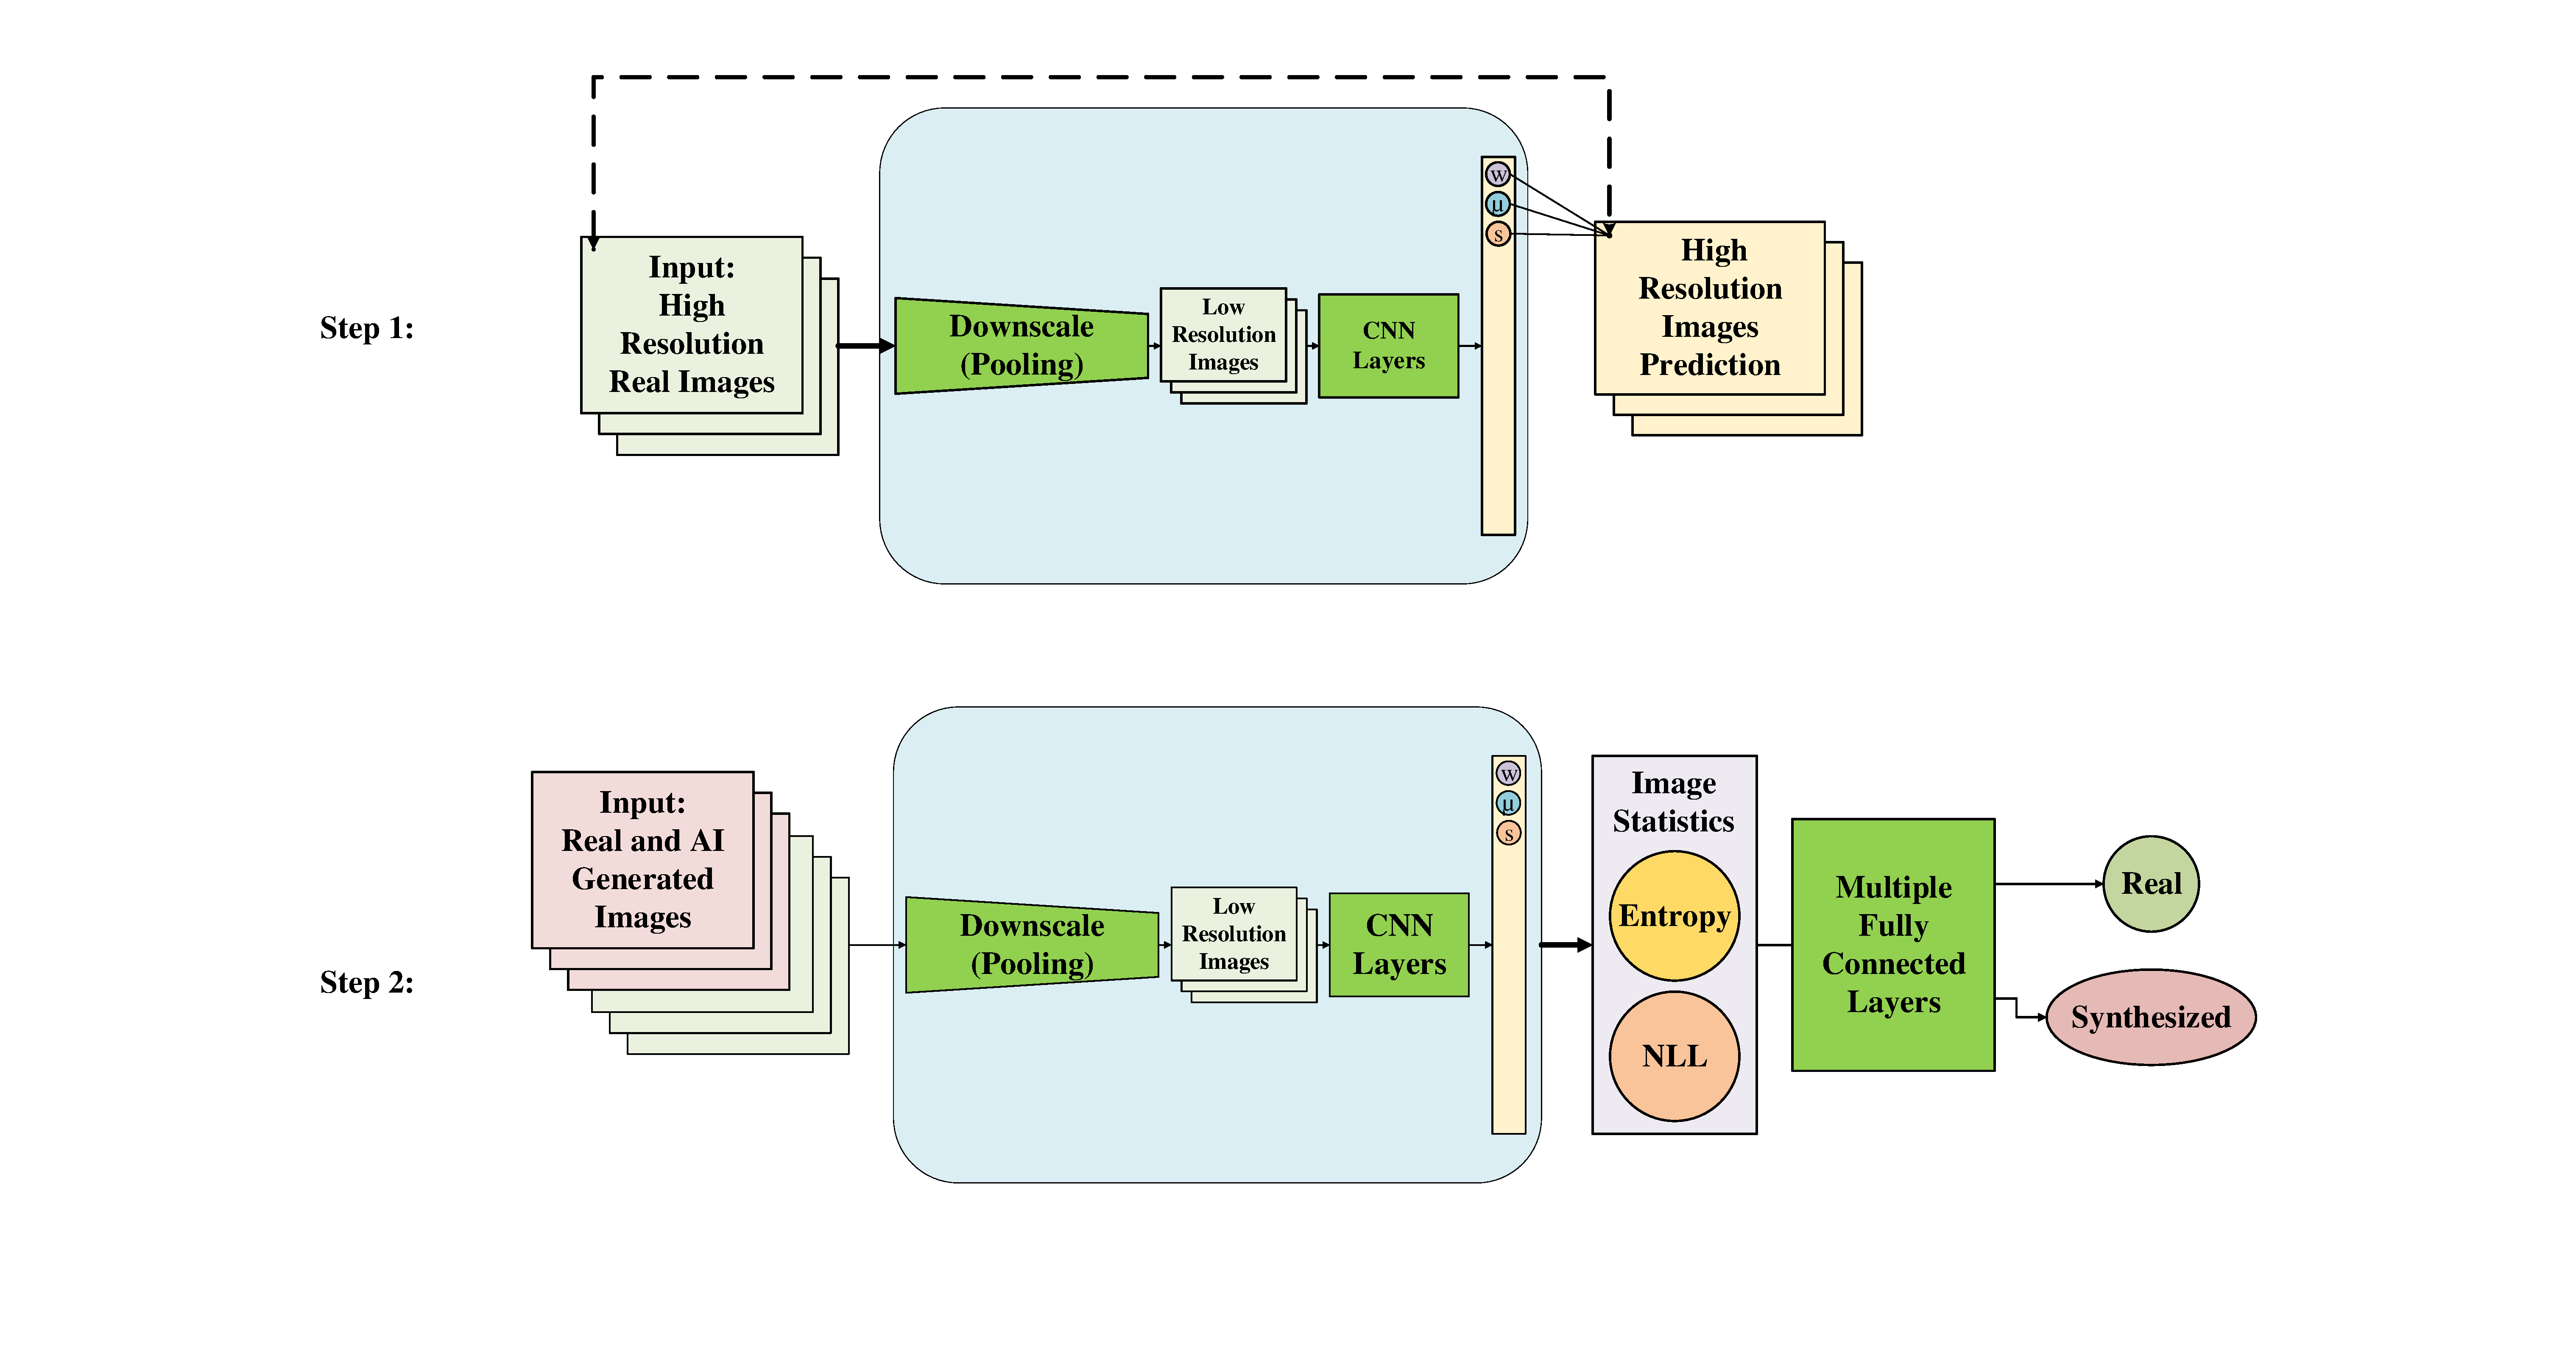
\includegraphics[width=\linewidth]{Fig/high_level_architecture.pdf}
    \caption{Figure1. Two-step high level architecture for AI-generated image detection. Step 1 (top) trains a compression and reconstruction model (blue box) solely on real images, learning to restore downscaled high-resolution images using CNN layers and logistic probability distribution parameters. Step 2 (bottom) applies the trained model (blue box) to both real and AI-generated images, extracting entropy-based statistics such as Negative Log-Likelihood (NLL) and entropy values. These statistics are passed through multiple fully connected layers for final classification.}
\end{figure}

\section{Background \& Related Work}
\label{background}

% 1. brief description of how images are generated (gan, dm)
Image synthesis is the process wherein an artificial image is generated by a computer from an input prompt, which may be text or some other form of media. This field exploded after the creation of Generative Adversarial Networks (GAN) in 2014, a deep learning architecture particularly adept at generating photorealistic images \citep{GANfather}. More recently, diffusion models (DM) have also been a popular choice for image synthesis \citep{latent-diffusion}. While many attempts have been made to develop programs that can detect images generated by these architectures, they continually evolve to outsmart old detectors.

\subsection{Sightengine}

There are a number of AI-generated image detection websites which are free to use. One of these is \citet{sightengine}, which has a high accuracy rate compared to many other websites: approximately 99\% on real images and 81\% on AI-generated ones \citep{li2024adversarialaiartunderstandinggeneration}. However, it is far from foolproof. For example, when tested on images generated from image prompts by Dream Studio and DALL-E, its accuracy falls to only 34\%. As opposed to images generated from text promts, images generated from real image prompts may be more challenging to detect, since they are more likely to be very similar to the real images they were generated from.

Many free websites like sightengine also predict the source of AI-generated images among many commonly-used synthesis models. Although the accuracy of this feature has not been formally investigated, it seems to fail often.

Though sightengine has not published its methods for AI-generated image detection, there are a number of open-source detectors available online, some of which are discussed below.

\subsection{Beyond the Spectrum}

Many earlier attempts at AI-generated image detection focused on GAN-generated images, since using DMs for image synthesis only began in 2022. One of these is Beyond the Spectrum (BtS), an open-source project \citep{he2021spectrumdetectingdeepfakesresynthesis}.

Its method for detection involves two stages. First, a re-synthesizer is trained, only on real images, to reconstruct images from their downsampled versions. Next, this re-synthesizer is given both real and fake images, and the reconstruction error (which is assumed to be greater for GAN-generated images) is given to a classifier to predict whether a given image is real or not.

In 2021, BtS achieved approxiately 90\% accuracy on its testing datasets and was state-of-the-art (SoTA). However, in 2024, after the progression of GAN models and the advent of DMs, BtS achieves only a 21\% accuracy rate \citep{li2024adversarialaiartunderstandinggeneration}. Nonetheless, its approach is echoed in more recent successful approaches, such as the zero-shot method discussed in \ref{ZED}.

\subsection{Contrastive Language–Image Pretraining}

Another architecture that has been explored for detecting AI-generated images is Contrastive Language–Image Pretraining (CLIP), which was developed by OpenAI in 2021 \citep{radford2021learningtransferablevisualmodels}. This model is trained on pairs of images and text, and in the context of AI-generated image detection, this text might either be their prompts or human-written descriptions. CLIP was used to achieve an accuracy of 95-100\% accuracy, making it a promising model for AI-generated image detection \citep{moskowitz2024detectingaigeneratedimagesclip}.

\subsection{Vision Transformers}

In natural language processing, text is interpreted as a sequence of tokens from which subsequent tokens can be predicted. Vision transformers (ViT) take a similar approach. Images are broken down into non-overlapping sections, like tokens, which are sent into an encoder comprised of multi-head attention and feed-forward neural networks. The output of the encoder is then passed into an MLP which classifies the image; in our case, it predicts whether the image is real or fake. In April 2024, researchers combined CLIP and ViT (CLIP-ViT) and were able to outperform a number of SoTA detection methods with an average accuracy of 90\% \citep{cozzolino2024raisingbaraigeneratedimage}.

\subsection{Zero-Shot Entropy-Based Detector}
\label{ZED}

The main issue in designing AI-generated image detectors is that image synthesis models are constantly evolving to circumvent detectors trained on old data. In September 2024, a new zero-shot method was devised which initally only trains on real images \citep{cozzolino2024zeroshotdetectionaigeneratedimages}. First, a CNN is trained to predict real images from encoded versions of those images. Next, the CNN is used to predict both real and fake images from their encoded versions, and loss statistics are fed into a classifier. Higher loss generally corresponds to AI-generated images, since the CNN provides a good model for real images.

This method was able to achieve an accuracy of 90\%, better than many other SoTA models. However, one drawback is that training and testing datasets were comprised only of uncompressed images.

\section{Data Processing}
\label{data}
In this project, three datasets are required: a training set, a testing set, and a validation set. As will be discussed in the following section, the Zero-Shot Entropy Detector (ZED) architecture is designed to be trained exclusively on real images, eliminating the need for synthetic data during training. To ensure that the model is generalizable to realworld data, and to avoid any issues like poor accuracy and overfitting, it is crucial to process training data so that all biases in the images are eliminated. The most impactful bias identified is the semantic content of images.
\subsection{Data Collection}
To guarantee that the model is exposed to a diverse range of semantics, we will utilize two well-established camera-based digital forensics datasets: 1. RAISE: A Raw Images Dataset For Digital Image Forensics; 2.The ‘Dresden Image Database’ For Benchmarking Digital Image Forensics. These datasets collectively contain approximately 22,000 real images, captured under varying conditions and environments. The model will be trained in two phases which will be mentioned in detail later. For the first phase, 10,000 real images will be allocated for training and 2,000 real images for validation. For the second phase, 5,000 real images will be allocated for training and 1,000 images for validation. The remaining 2,000 real images will be reserved for evaluation in the testing phase. For the second phase, 5,000 synthetic images will also be used to training and 1,000 for validation which enables the model to develop a robust entropy-based understanding of real-world image statistics.
The testing dataset will be balanced, comprising 2,000 real images and 2,000 AI-generated images. The synthetic images will be sourced from the SyntheticEye AI-Generated Image Dataset [SyntheticEye Reference], which includes images produced by a range of state-of-the-art generative models, including Stable Diffusion, DALL·E, and others. Incorporating AI-generated images from multiple sources ensures that the testing conditions closely reflect real-world inputs, enhancing the model’s ability to generalize across diverse synthetic image distributions.

\subsection{Data Modification}
For image inputs, the CNN requires a fixed resolution of 256×256 pixels. To ensure compatibility, all images in both the training and testing datasets will be cropped to 256×256 while preserving their essential features.
Additionally, to prevent any biases arising from variations in image attributes, all datasets will be normalized and standardized. This includes converting all images to RGB color space, ensuring uniform channel distributions across the dataset. Standardizing the color format enhances consistency in feature representation, improving the model's robustness and generalization.

\section{Architecture}
\label{arch}
\subsection{Motivation}
Nowadays, image classification models typically use Convolutional Neural Network (CNN) as their base architecture. Classical CNNs will use datasets that consists of AI-generated images to train and learn special attributes about these artificial pictures. But inefficiencies in the training process of CNNs are starting to surface as more and more image generation models are being released. With more image generation models come different characteristics that the CNN classifier never learned. This leads towards a need for training with the new datasets which both takes time and money (Cozzolino et al. 2024).

The Zero-Shot Entropy Detector(ZED) is unique in a way that its training process for detecting AI-generated images doesn’t rely on synthetic data sets. The main idea behind ZED is to estimate how “surprising” an image is compared to the real images it trained on. It is assumed that real images follow a “natural” statistic pattern, while AI-generated images typically consists of “unnatural” statistical patterns that are detectable \citep{cozzolino2024zeroshotdetectionaigeneratedimages}.

% entropy and nll based, so maybe it's image statistic based?
% we did used ai images in the second step training
% I think we need to mention nll entropy is enough to detemine if a image is ai generated from the zed paper
\subsection{Architecture}
The architecture of our neural network consists of two phases: CNN training and entropy based classification. In the CNN, a real image is first fed into a CNN where a predicted representation of the image is outputted. The error between the predicted and expected output would be back propagated to adjust the weights and biases through the layers of neurons. After the CNN is trained, it will be connected to a classifier where entropy based loss would be used to predict whether an image is AI-generated or real. This approach allows for zero-shot generalization, meaning the system can detect new AI-generated images without explicit training on synthetic data.



\section{Baseline Model}
\label{baseline}
% resnet is too complicate for baseline model

% I will revise after reading the data processing section to give more specific numbers for dataset sizes
Our baseline model will mirror \citet{wang2020cnngeneratedimagessurprisinglyeasy}, an early attempt at AI-generated image detection. This model uses ResNet-50 trained on real images from ImageNet and fake images generated by three GAN architecures. We will expand our dataset to include fake images from a greater variety of image generators, including diffusion models (see \ref{data}). For simplicity, we will use a CNN but not ResNet. Like \citet{wang2020cnngeneratedimagessurprisinglyeasy}, the classifier will use a binary cross-entropy loss function.

\section{Ethical Considerations}
\label{ethical}

Ethical considerations here

\section{Project Plan}
\label{plan}

Team communication will be crucial to our success. Our main channel of communication will be a Whatsapp group chat, which we have used thus far. We will meet once every Sunday at 10am, but should we need to meet more frequently, we will use our chat to determine meeting times on a rolling basis.

To ensure team cohesion and clear delineation of tasks, we will (a) assign specific tasks to each team member as explained in \ref{assigning_work} and (b) use Git for version control.

\subsection{Assigning Work}
\label{assigning_work}

For written deliverables, we will all brainstorm ideas and points for each section. However, to ensure that we do not overwrite each other's work, each team member will be responsible for drafting certain sections. The point total of one member's assigned sections should be similar to the totals of every other team member's assigned sections to ensure equal work. We will use Git for version control so that we can clearly see the contributions of each team member. Using LaTeX comments, our group chat, and verbal communication, we will notify each other of suggestions that we have for each other's work.

Regarding work on the project itself, we will equally delineate ``substantial tasks'' as described in the Project Final Report Handout and Rubric CITE (see \ref{detailed_plan}). This we will ensure that we are not overwriting each other's work and that we each share an equal load of the total work. Like with written deliverables, we will use comments, our group chat, and verbal communication to share suggestions for each other's work.

\subsubsection{Project Proposal}

Table \ref{project_proposal_table} shows who is responsible for drafting each section of the Project Proposal. Note that each member is assigned between 9 and 11 points.

    \begin{table}[t]
    \caption{Project Proposal task assignment and deadlines.}
    \label{project_proposal_table}
    \begin{center}
    \begin{tabular}{llll}
    \multicolumn{1}{c}{\bf Task}                    & \multicolumn{1}{c}{\bf Points} & \multicolumn{1}{c}{\bf Internal Deadline} & \multicolumn{1}{c}{\bf Assignee(s)}
    \\ \hline \\
    Introduction                                    & 4                              & 02-06                                     & Vedansh \\
    Creating Illustration/Figure                    & 4                              & 02-06                                     & William \\
    Background \& Related Work                      & 4                              & 02-06                                     & Nathan \\
    Data Processing                                 & 4                              & 02-06                                     & Paul \\
    Architecture                                    & 2                              & 02-06                                     & Paul \\
    Baseline Model                                  & 2                              & 02-06                                     & Paul \\
    Ethical Considerations                          & 2                              & 02-06                                     & William \\
    Risk Register                                   & 4                              & 02-06                                     & Vedansh \\
    Project Plan                                    & 4                              & 02-06                                     & Nathan \\
    GitHub \& Colab Repositories                    & 1                              & 02-06                                     & William \\
    Formatting References                           & 1                              & 02-06                                     & Nathan \\
    Proofreading (Structure, Grammar, Mechanics)    & 8                              & 02-06                                     & All Members \\
    \end{tabular}
    \end{center}
    \end{table}

\subsubsection{Detailed Plan}
\label{detailed_plan}

Table \ref{plan_table} shows our internal deadlines for various components of the project throughout the rest of the semester. Though we will each work on all aspects of the projects, each aspect will be spearheaded by certain group members.

    \begin{table}[t]
    \caption{Project internal deadlines.}
    \label{plan_table}
    \begin{center}
    \begin{tabular}{llll}
    \multicolumn{1}{c}{\bf Task}            & \multicolumn{1}{c}{\bf Internal Deadline} & \multicolumn{1}{c}{\bf Task Lead(s)}
    \\ \hline \\
    Data Collection \& Verification         & 02-23                                     & Paul \& Vedansh \\
    Data Preprocessing                      & 03-01                                     & Paul \& Vedansh \\
    Baseline Model Implementation           & 03-01                                     & Nathan \& Paul \\                   
    Primary Model Design                    & 03-16                                     & Nathan \& William \\
    Primary Model Training \& Optimization  & 03-25                                     & Nathan \& William \\
    Primary Model Analysis                  & 03-30                                     & Vedansh \& William \\
    \end{tabular}
    \end{center}
    \end{table}
    

\section{Risk Register}
\label{risk}

Risk register here

\label{last_page}

\bibliography{APS360_ref}
\bibliographystyle{iclr2022_conference}

\end{document}
